\newpage
\phantomsection
{\bfseries МРНТИ 38.33.25}
\hfill {\bfseries \href{https://doi.org/10.58805/kazutb.v.2.23-379}{https://doi.org/10.58805/kazutb.v.2.23-379}}

\sectionwithauthors{Р.К. Мадишева, Г.М. Жексенбаева, Р.К. Адилханов, А.Б. Демеуова, Г.Б. Амангельдиева, М.Б. Умирзакова}{НЕФТЕМАТЕРИНСКИЙ ПОТЕНЦИАЛ ЮРСКИХ ОТЛОЖЕНИЙ АРЫСКУМСКОГО ПРОГИБА ЮЖНО-ТОРГАЙСКОГО БАССЕЙНА}

\begin{center}
{\bfseries \textsuperscript{1}Р.К. Мадишева, \textsuperscript{1}Г.М. Жексенбаева\envelope, \textsuperscript{1}Р.К. Адилханов, \textsuperscript{1}А.Б. Демеуова, \textsuperscript{1}Г.Б. Амангельдиева, \textsuperscript{2}М.Б. Умирзакова}

\textsuperscript{1}Некоммерческое акционерное общество «Карагандинский
технический университет имени Абылкаса Сагинова», Караганда, Казахстан,

\textsuperscript{2}Акционерное общество «КазАзот» филиал «Шагырлы --
Шомышты»,

\envelope Корреспондент-автор: Gulmira\_zh91@mail.ru
\end{center}

Цель данного исследования заключается в изучении и оценке
нефтематеринского потенциала пород мезозойских отложений Арыскумского
прогиба методом Rock-Eval. Результаты анализа методом пиролиза позволяют
получить несколько важных показателей, связанных с формированием нефти,
таких как содержание свободных углеводородов, остаточное содержание
углеводородов, уровень термической зрелости образца, количество
химически активного органического вещества. Для достижения поставленной
цели выполнялись следующие задачи: 1. Оценка нефтегенеративного
потенциала; 2. Определение стадии термической зрелости органического
вещества и типа керогена.

По результатам геохимических исследований органического вещества
установлено, что концентрации общего органического углерода (TOC) в
образцах пород указывает на различный генеративный потенциал этих пород,
охватывая диапазон от бедного до богатого. Это свидетельствует о
потенциале этих пород для генерации углеводородов. Значения
T\textsubscript{max}, которые позволяют оценить термическую зрелость
органического вещества и его способность к нефтегенерации,
свидетельствуют о том, что органическое вещество исследуемых образцов
может быть классифицировано как зрелое с возможностью генерации нефти и
низкой степенью зрелости. Параметр S\textsubscript{1}+S\textsubscript{2}
позволил классифицировать исследованные образцы как нефтегенерирующие с
умеренным потенциалом и газогенерирующие.

Эти выводы подчеркивают важность геохимических исследований
органического вещества и пиролитического анализа пород для оценки их
генетического, нефтегазоносного и зрелостного потенциала.

{\bfseries Ключевые слова:} пиролиз, нефтематеринские породы, Арыскумский
прогиб, органическое вещество, тип керогена.

\begin{center}
{\large\bfseries ОҢТҮСТІК ТОРҒАЙ БАССЕЙНІНІҢ АРЫСҚҰМ ИІЛІМДЕГІ ЮРА ШӨГІНДІЛЕРІНІҢ
МҰНАЙАНАЛЫҚ ПОТЕНЦИАЛЫ}

{\bfseries \textsuperscript{1}Р.К. Мадишева, \textsuperscript{1}Г.М.
Жексенбаева\envelope, \textsuperscript{1}Р.К. Адилханов,
\textsuperscript{1}А.Б. Демеуова,\\
\textsuperscript{1}Г.Б. Амангельдиева, \textsuperscript{2}М.Б.
Умирзакова}

\textsuperscript{1}«Әбілқас Сағынов атындағы Қарағанды техникалық
университеті» коммерциялық емес акционерлік қоғамы, Қарағанды,
Қазақстан,

\textsuperscript{2}«КазАзот» акционерлік қоғамы «Шагырлы -- Шомышты»
филиалы, Қарағанды, Қазақстан,

e-mail: Gulmira\_zh91@mail.ru
\end{center}

Бұл зерттеудің мақсаты-Rock-Eval әдісімен Арысқұмның мезозой шөгінділері
жыныстарының мұнайаналық потенциалын зерттеу және бағалау. Пиролиз
әдісімен талдау нәтижелері мұнайдың түзілуіне байланысты бірнеше маңызды
көрсеткіштерді алуға мүмкіндік береді, мысалы, бос көмірсутектердің
мөлшері, көмірсутектердің қалдық мөлшері, үлгінің термиялық жетілу
деңгейі, химиялық белсенді органикалық заттардың мөлшері. Мақсатқа жету
үшін келесі міндеттері орындалды: 1. Мұнайдың генеративті потенциалын
бағалау; 2. Органикалық заттардың термиялық жетілу кезеңін және кероген
түрін анықтау.

Органикалық заттардың геохимиялық зерттеулерінің нәтижелері бойынша тау
жыныстарының үлгілеріндегі жалпы органикалық көміртектің (TOC)
концентрациясы кедей көрсеткіштен бай көрсеткішке дейінгі диапазонды
қамтитын осы жыныстардың әртүрлі генеративті потенциалын көрсететіні
анықталды. Бұл осы тау жыныстарының көмірсутектерді өндіру потенциалын
көрсетеді. Органикалық заттардың термиялық жетілуін және оның мұнай
өндіру қабілетін бағалауға мүмкіндік беретін T\textsubscript{max}
мәндері зерттелетін үлгілердің органикалық заттарын мұнай өндіру
мүмкіндігімен және төмен жетілу дәрежесімен жетілген деп жіктеуге
болатынын көрсетеді. S\textsubscript{1}+S\textsubscript{2} параметрі
зерттелген үлгілерді орташа потенциалды мұнай өндіретін және газ
өндіретін деп жіктеуге мүмкіндік берді.

Бұл тұжырымдар органикалық заттардың геохимиялық зерттеулерінің және
олардың генетикалық, мұнай-газ және жетілу потенциалын бағалау үшін тау
жыныстарын пиролитикалық талдаудың маңыздылығын көрсетеді.

{\bfseries Түйін сөздер:} пиролиз, мұнайаналық жыныстар, Арысқұм иілімі,
органикалық заттар, кероген түрі.

\begin{center}
{\large\bfseries THE OIL-PRODUCING POTENTIAL OF THE JURASSIC DEPOSITS OF THE
ARYSKUM DEPRESSION OF THE SOUTH TORGAI BASIN}

{\bfseries \textsuperscript{1}R.K. Madisheva, \textsuperscript{1}G.M.
Zhexenbayeva\envelope, \textsuperscript{1}R.K. Adilkhanov,
\textsuperscript{1}A.B. Demeuova,}

{\bfseries G.B. Amangeldiyeva\textsuperscript{1}, M.B.
Umirzakova\textsuperscript{2}}

\textsuperscript{1}Non-profit Joint Stock Company «Abylkas Saginov
Karaganda Technical University», Karaganda, Kazakhstan,

\textsuperscript{2} Joint Stock Company «KazAzot» branch «Shagyrly --
Shomyshty», Karaganda, Kazakhstan,

e-mail: Gulmira\_zh91@mail.ru
\end{center}

The purpose of this study is to study and evaluate the oil source
potential of the Mesozoic rocks of the Aryskum depression using the
Rock-Eval method. The results of analysis by pyrolysis method allow us
to obtain several important indicators related to the formation of oil,
such as the content of free hydrocarbons, residual hydrocarbon content,
the level of thermal maturity of the sample, and the amount of reactive
organic matter. To achieve this goal, the following tasks were
performed: 1. Assessment of oil-generating potential; 2. Determination
of the stage of thermal maturity of organic matter and the type of
kerogen.

Based on the results of geochemical studies of organic matter, it was
found that the concentration of total organic carbon (TOC) in rock
samples indicates the different generative potential of these rocks,
covering the range from poor to rich. This indicates the potential of
these rocks to generate hydrocarbons. The T\textsubscript{max} values,
which allow us to assess the thermal maturity of organic matter and its
ability to generate oil, indicate that the organic matter of the studied
samples can be classified as mature with the ability to generate oil and
a low degree of maturity. The S\textsubscript{1}+S\textsubscript{2}
parameter made it possible to classify the studied samples as
oil-generating with moderate potential and gas-generating.

These findings highlight the importance of geochemical studies of
organic matter and pyrolytic analysis of rocks to assess their genetic,
petroleum and maturity potential.

{\bfseries Keywords:} pyrolysis, oil source rocks, Aryskum depression,
organic matter, kerogen type.

\begin{multicols}{2}
{\bfseries Введение.} Исследование методом пиролиза---это важный инструмент
для геохимического анализа горных пород, используемый
геохимиками-нефтяниками. В данной методике применяется программируемый
пиролиз с открытой системой, при котором применяются ступенчатые режимы
нагрева к тщательно подготовленным образцам между заданными
температурными порогами. Первоначально образцы подвергаются пиролизу в
инертной атмосфере, что позволяет образоваться нефтяным флюидам, а затем
происходит их окисление в окисляющей среде. Метод обладает несколькими
ключевыми преимуществами: 1) обеспечивает быстрое получение полезных
измерений, характеризующих исходную породу; 2) потребляет очень малое
количество пробы во время анализа, что делает его привлекательным для
исследования керна скважин и шлама {[}1{]}.

Результаты анализа позволяют получить нескольких важных показателей,
связанных с формированием нефти, таких как содержание свободных
углеводородов, остаточное содержание углеводородов, уровень термической
зрелости образца, количество химически активного органического вещества,
присутствие карбонатных минералов и качество органического вещества
{[}2{]}.

Геологическая характеристика. Южно-Торгайский бассейн имеет
северо-западное направление и занимает площадь 8×10\textsuperscript{4}
км\textsuperscript{2}. Он представляет собой рифтовую депрессию,
расположенную между Нижнесырдарьинским сводом и массивом Улытау. На
сегодняшний день в бассейне обнаружено более 50 месторождений нефти и
газа. Промышленная нефтегазоносность этого региона доказана в 1984 году
после обнаружения фонтана нефти в первой поисковой скважине на площади
Кумколь {[}3, 4{]}.

По особенностям структурного плана в бассейне выделяются две области
прогибания - Арыскумский и Жыланшикский прогибы и разделяющая их
Мынбулакская седловина. Арыскумский прогиб характеризуется высокой
концентрацией углеводородов на единицу площади. Геологическая структура
прогиба представлена двухъярусной структурой - на нижнем уровне
преобладают глубокие грабены, состоящие из терригенных юрских отложений,
и между ними находятся горстообразные выступы, представленные формациями
доюрского возраста {[}5{]}. Вершины палеозойских выступов могут состоять
из разрушенных пород, что создает условия для образования нефтегазовых
месторождений. На верхнем уровне прогиба преобладают терригенные породы,
в основном мелового и кайнозойского возраста, которые покрывают более
древние отложения (Рисунок. 1).

Глубина фундамента уменьшается в северном направлении, и наибольшая
глубина наблюдается в центральной части Южно-Торгайского бассейна в
районе разлома Каратау {[}6{]}.
\end{multicols}

\begin{figure}[H]
	\centering
	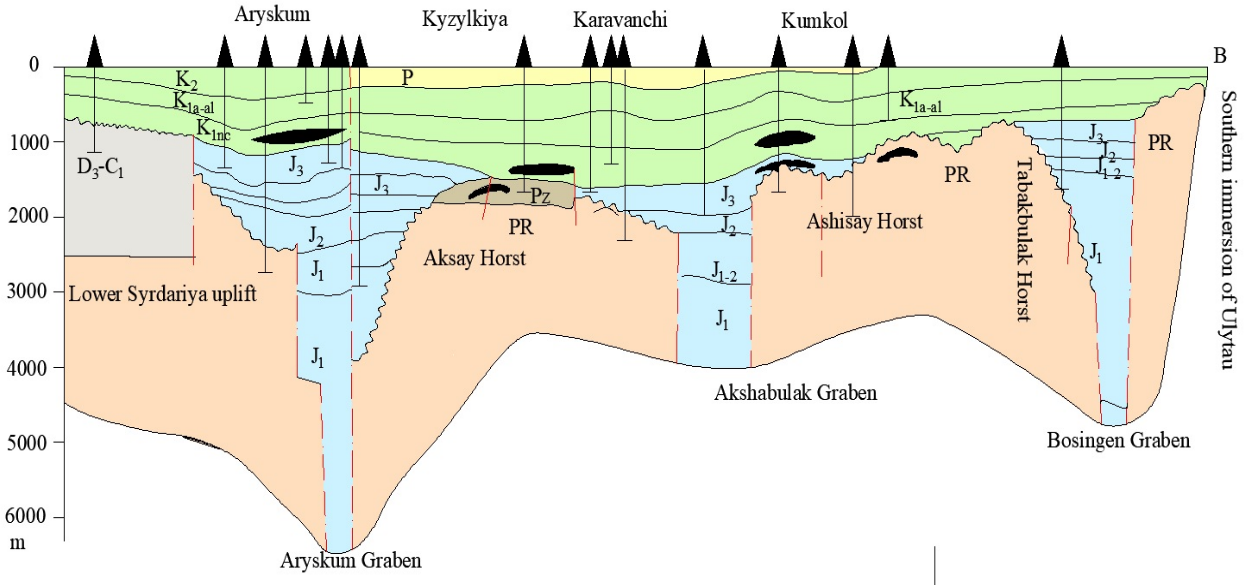
\includegraphics[width=0.9\textwidth]{assets/1258}
	\caption*{Рис. 1 - Геологический профиль Южно-Торгайского бассейна {[}6{]}}
	\caption*{Условные обозначения: J\textsubscript{1}--нижняя юра, J\textsubscript{2}--средняя юра, J\textsubscript{3}--верхняя юра, K\textsubscript{1}a-al--нижний мел, K\textsubscript{2}--верхний мел, Pz--палеозой, PR--протерозой, D\textsubscript{3}-C\textsubscript{1}--верхний девон-нижний карбон}
\end{figure}

\begin{multicols}{2}
{\bfseries Материалы и методы.} Геохимические исследования органического
вещества включают пиролитический анализ, проводимый на анализаторе
Source Rock Analyzer (SRA-TPH/TOC) в лаборатории Weatherford
Laboratories Instruments Division's. В ходе анализа керн измельчается и
просеивается через 40-mesh ситу. Далее определяется количество свободных
углеводородов (S\textsubscript{1}) и нелетучих органических веществ
(S\textsubscript{2}) в миллиграммах на грамм породы. Также проводится
измерение общего органического углерода (TOC) и температура
(T\textsubscript{max}) во время пиролиза, при которой происходит
максимальное высвобождение углеводородов из трещин керогена. Эти данные
необходимы для получения информации о нефтегазоносности породы и ее
потенциальной способности к генерации углеводородов {[}7{]}.

{\bfseries Результаты и обсуждения.} Цикл окисления следует за циклом
пиролиза, в ходе которого образцы сжигаются в присутствии кислорода. Для
встроенной программы Rock-Eval существуют различные методы, такие как
«основной метод/метод насыпных пород» и «метод чистого органического
вещества», которые могут быть выбраны в зависимости от типа
анализируемого образца. При использовании метода «основной/насыпной
породы», образец сначала выдерживается в изотермическом режиме при
температуре 300°C в течение 3 минут (Рисунок. 2) {[}8{]}.
\end{multicols}

\begin{figure}[H]
	\centering
	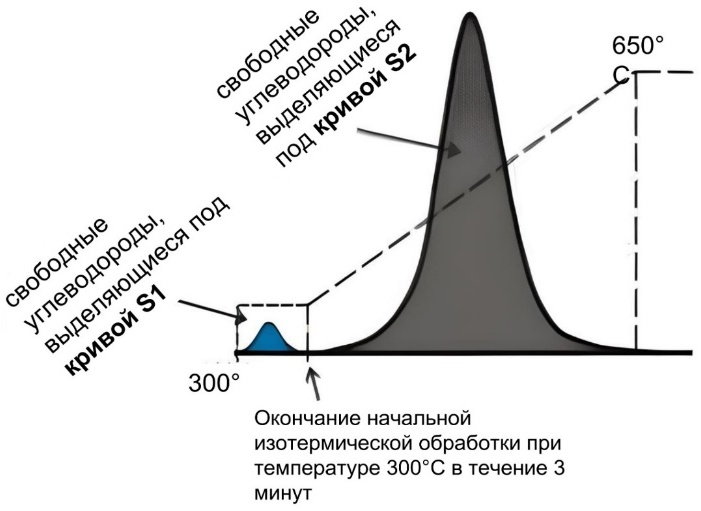
\includegraphics[width=0.5\textwidth]{assets/1259}
	\caption*{Рис. 2 - Обобщенная диаграмма, показывающая пики оценки горных пород от S\textsubscript{1} до S\textsubscript{2}, обычно полученные с использованием базового метода оценки горных пород}
\end{figure}

\begin{multicols}{2}
Во время данной фазы, свободные молекулы углеводородов или те, которые
легко испаряются или слабо связаны с матрицей образца, высвобождаются,
образуя пар, который регистрируется как составляющий кривую
S\textsubscript{1} оценки породы. Такой выделяющийся пар обнаруживается
ионизационным детектором (FID). После 3-минутной начальной
изотермической стадии, образцы нагреваются в течение цикла пиролиза
систематически небольшими равномерными шагами по шкале нагрева от 300°C
до заданной конечной температуры (650°C или 800°C).

Во время этой второй стадии пиролиза происходит доступ к молекулам
углеводородов и структурам органического вещества или керогена, их
высвобождение и расщепление на более мелкие и летучие молекулы
углеводородов. При подобных более высоких температурах, аналогичных
температурам, используемым в процессах крекинга на нефтеперерабатывающих
заводах, более тяжелые пиролизаты, содержащиеся в керогене,
высвобождаются и превращаются в пар. Эти пары снова обнаруживаются FID и
записываются для построения кривой S\textsubscript{2}. Таким образом,
значения S\textsubscript{2} указывают на остаточную способность образца
к образованию нефти, то есть количество нефти, которое мог бы произвести
образец, если бы он был взят естественным путем в течение геологического
времени через полный цикл термического созревания (в зону термической
зрелости сухого газа).

Подробные характеристики формы и температуры пика S\textsubscript{2}
широко используются для классификации нефтеобразующего потенциала
керогенов. Максимумы температуры, при которых образуется максимальное
количество пиролизатов в пределах S\textsubscript{2}, пиковые значения
обозначаются как T\textsubscript{max}, который широко используется в
качестве показателя термической зрелости (Рисунок. 3). Чем более
термически зрел образец, тем более стабильными становятся его остаточные
углеводородные фрагменты (или молекулярные компоненты), то есть, те,
которые остаются после того, как летучие или похожие на нефть молекулы
удаляются как часть пика S\textsubscript{1}. Остаточные углеводородные
фрагменты требуют более высоких температур для расщепления и образования
дополнительных молекул, связанных с нефтью. Значительным улучшением
Rock-Eval 6 по сравнению с более ранними моделями является расположение
датчика, контролирующего температуру пиролиза {[}6, 9{]}.

Максимальный параметр в Rock-Eval 6, таким образом, является
произвольным показателем зрелости, применяемым к температурному пику
S\textsubscript{2}, и не отражает истинную температуру, а используется
только для обеспечения единообразия в геохимической классификационной
схеме для аналитиков. Показатель T\textsubscript{max}, с другой стороны,
рассчитывается таким образом, чтобы получить приблизительно одинаковое
значение для конкретного образца при различных скоростях нагрева, и,
таким образом, обеспечивает полезный показатель термической зрелости
этого образца {[}6, 10{]}.

Форма пирограмм S\textsubscript{2} дает представление о типе керогена и
его термической зрелости: кероген I типа обладает высоким потенциалом
образования углеводородов. В то время как кероген III-IV типов имеет
более низкий потенциал образования нефти. Также стоит учитывать, что
мигрировавшие углеводороды в образцах могут оказывать влияние на оценку
породы, основанную на полученных пирограммах.

Количество органического вещества в горных породах, керогене, а также
присутствие углеводородов в образце определяются параметром общего
органического углерода (TOC), и относительная способность исходной
породы генерировать углеводороды зависит от качества и количества
органического вещества.

Результаты геохимического исследования, представлены в таблице 1, где
концентрация общего органического углерода (TOC) варьирует от 0,47\% до
1,41\%. Образцы с низкими значениями TOC (\textless0.5) были исключены
из анализа для корректной интерпретации данных пиролиза. Согласно
классификации нефтегазоматеринских пород, исследованные образцы обладают
генеративным потенциалом от плохого (бедного) до хорошего (богатого) в
зависимости от концентрации TOC. Представленные в таблице 1 результаты
геохимического анализа образцов каменного материала кумкольской свиты
верхней юры (J\textsubscript{3}km) и арыскумской свиты нижнего мела
(K\textsubscript{1}nc\textsubscript{1}ar) свидетельствуют о том, что
концентрация общего органического углерода (ТОС) варьирует от 0.47 до
1.41 \% {[}6, 11{]}.
\end{multicols}

\begin{table}[H]
\caption*{Таблица 1 - Геохимическая характеристика по пиролитическому анализу отложений Арыскумского прогиба Южно-Торгайского бассейна, Казахстан}
\centering
\begin{tabular}{|l|l|l|l|l|l|l|l|l|l|}
\hline
№ & Formation & Depth & TOC & S\tsb{1} & S\tsb{2} & S\tsb{1}+S\tsb{2} & T\tsb{max} & S\tsb{1}/TOC & OSI \\ \hline
1 & K\tsb{1}nc\tsb{1}ar & 1682.9 & 0.52 & 0.97 & 1.6 & 2.57 & 413.02 & 0.187 & 187 \\ \hline
2 & K\tsb{1}nc\tsb{1}ar & 1686.4 & 0.53 & 0.57 & 2.2 & 2.77 & 437.49 & 0.108 & 108 \\ \hline
3 & K\tsb{1}nc\tsb{1}ar & 1687.43 & 1.12 & 02.05 & 3.1 & 5.15 & 445.16 & 0.183 & 183 \\ \hline
4 & J\tsb{3}km & 1880.45 & 0.67 & 0.3 & 2.6 & 2.9 & 434.19 & 0.045 & 45 \\ \hline
5 & J\tsb{3}km & 1883.85 & 0.47 & 0.24 & 1.1 & 1.34 & 440.33 & 0.051 & 51 \\ \hline
6 & J\tsb{3}km & 1887.67 & 0.57 & 0.37 & 2.3 & 2.67 & 432.6 & 0.065 & 65 \\ \hline
7 & J\tsb{3}km & 1896.54 & 0.68 & 0.49 & 2.8 & 3.29 & 330.67 & 0.072 & 72 \\ \hline
8 & J\tsb{3}km & 1897.19 & 0.71 & 0.22 & 2 & 2.22 & 437.8 & 0.031 & 31 \\ \hline
9 & J\tsb{3}km & 1897.36 & 1.41 & 1.65 & 9 & 10.65 & 434.11 & 0.117 & 117 \\ \hline
\end{tabular}
\end{table}

\begin{multicols}{2}
Исходя из этой информации, можно сделать вывод, что образцы
нефтегазоматеринских пород, у которых концентрация общего органического
углерода (TOC) ниже 0,5\%, были исключены из анализа. Это позволило
правильно интерпретировать данные пиролиза, так как количество
органического вещества существенно влияет на потенциал породы для
генерации нефти. Также, исходя из классификации нефтегазоматеринских
пород, можно сделать вывод, что исследованные образцы обладают
потенциалом от плохого (бедного) до хорошего (богатого), и это связано с
различными концентрациями общего органического углерода (TOC) {[}6{]}.

Хант предложил использовать отношение S\textsubscript{1} к содержанию
органического углерода (TOC) для выделения мигрировавших углеводородов
или загрязняющих веществ в образце. Значения коэффициента
S\textsubscript{1}/TOC\textgreater1,5 указывают на присутствие
мигрировавших углеводородов или загрязняющих веществ, в то время как
значения менее 1,5 указывают на присутствие коренных углеводородов или
углеводородов in situ. Индекс нефтенасыщенности (OSI), рассчитываемый
как (S\textsubscript{1}/TOC)*100, должен превышать 100 мг HC/г TOC для
насыщенных сланцев. Однако, OSI\textgreater150 мг HC/г TOC указывает на
наличие в образце загрязнений, связанных с бурением, или мигрировавшей
нефти. Эти методы являются важным инструментом для оценки наличия нефти
и других углеводородов в породах {[}12, 13{]}.

Количество углеводородов, выделяемых во время термического пиролиза
(параметр S\textsubscript{2}), играет важную роль в определении
нефтепродуктивного потенциала породы (Рисунок 3.).
\end{multicols}

\begin{figure}[H]
	\centering
	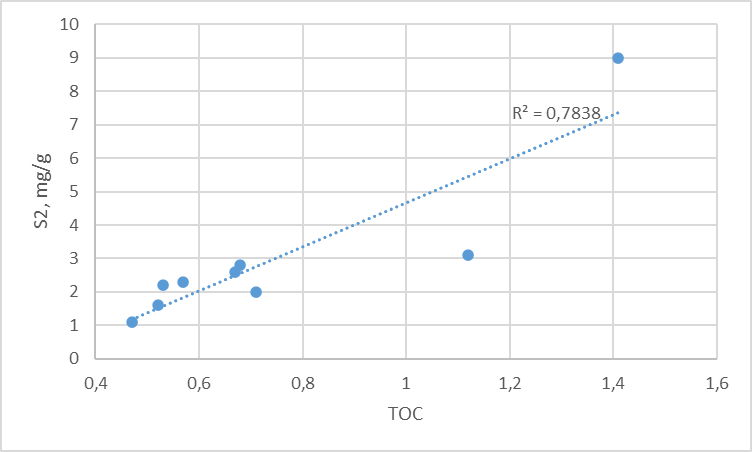
\includegraphics[width=0.6\textwidth]{assets/1260}
	\caption*{Рис. 3 - График зависимости TOC от параметра S\textsubscript{2}}
\end{figure}

\begin{multicols}{2}
График зависимости TOC от S\textsubscript{2} демонстрирует линейную
связь и имеет коэффициент корреляции R\textsuperscript{2}=0,7838. В
изучаемых образцах даульской свиты нижнего мела параметр
S\textsubscript{2} находится в диапазоне от 1.6 до 3.1 мг УВ/г породы, в
то время как для кумкольской свиты верхней юры значения
S\textsubscript{2} колеблются от 1.1 до 9 мг УВ/г породы. Значения
S\textsubscript{2} ниже 2.5 указывают на низкий потенциал, а выше 6 - на
высокий потенциал генерации углеводородов.

Определение термической зрелости. Значения T\textsubscript{max}
предоставляют возможность оценить термическую зрелость органического
вещества и его способность к нефтегенерации в породах. Диапазон значений
T\textsubscript{max} для исследуемых образцов от 435 до 445°C
соответствует условиям нефтяного окна, что указывает на возможность
генерации нефти и позволяет отнести их к зрелым. Низкие значения
T\textsubscript{max} (менее 435°C) для образцов керна с глубины 1682,9 м
(даульская свита) и 1896,54 м (кумкольская свита) указывают на невысокую
степень зрелости органического вещества, как показано на рисунке 4
{[}14{]}.
\end{multicols}

\begin{figure}[H]
	\centering
	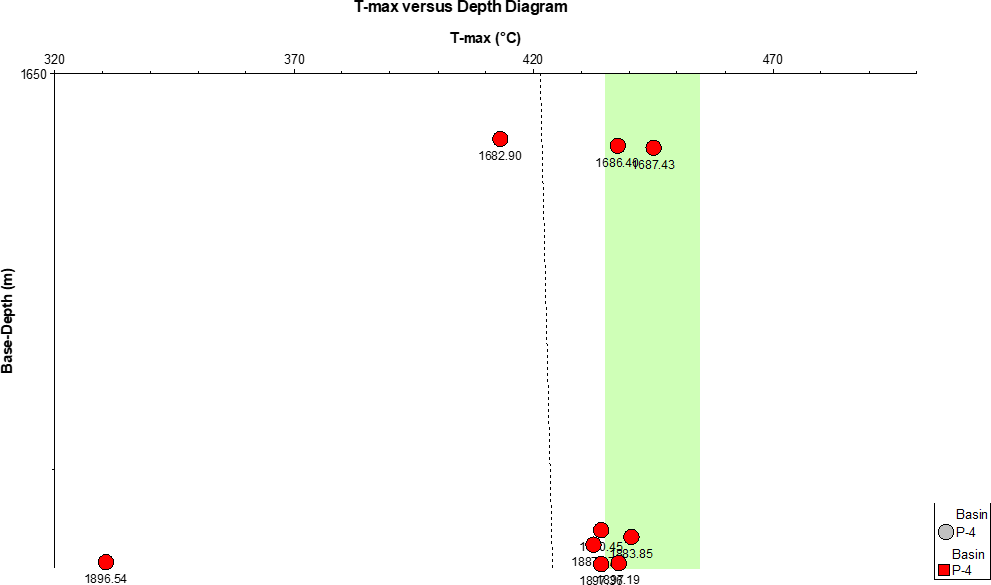
\includegraphics[width=0.6\textwidth]{assets/1261}
	\caption*{Рис. 4 - Диаграмма зависимости T\textsubscript{max} от глубины Арыскумского прогиба Южно-Торгайского бассейна, Казахстан}
\end{figure}

\begin{multicols}{2}
Важные показатели и критическая информация, касающаяся функционирования
системы оценки горных пород для оценки пород-источников и коллекторов.
Оценка породы S\textsubscript{1}: Наличие или отсутствие углеводородов,
связанных с нефтью, может быть определено через пик S\textsubscript{1},
который указывает на наличие газа, жидкости или твердых углеводородных
соединений в исследуемом образце. Однако, важно учитывать, что некоторые
из этих углеводородов могут быть доставлены в изучаемый пласт
естественными процессами миграции нефти из других частей месторождения.
Таким образом, при интерпретации пика S\textsubscript{1} следует
учитывать не только местные углеводороды, но и возможность миграции и
перераспределения углеводородов внутри пласта, что подчеркивает важность
глубокого анализа и многогранных подходов к интерпретации геохимических
данных. Более того, пики S\textsubscript{1} в образцах из ствола
скважины могут содержать примеси, которые присутствуют в буровом
растворе, особенно если используются буровые растворы на нефтяной
основе. Эти углеводородные примеси в основном расщепляются при пиролизе,
что может привести к ложно завышенным значениям пика S\textsubscript{1}.
Кроме того, остатки этих примесей могут оказать влияние на пик
S\textsubscript{2}, измеряемый в породах, а также на его значения
T\textsubscript{max} {[}15, 16{]}.

Сумма S\textsubscript{1}+S\textsubscript{2} (в миллиграммах УВ на грамм
породы) для образца может использоваться для определения генетического
потенциала породы. В данном контексте, значение этой суммы позволяет
классифицировать породы как нефтегенерирующие с умеренным потенциалом,
за исключением образца кумкольской свиты с глубиной 1883,85 м, у
которого сумма S\textsubscript{1}+S\textsubscript{2} менее 2 мг/г, что
вероятнее всего указывает на его не нефтегенерирующий характер. По
диапазону значений S\textsubscript{1}+S\textsubscript{2} от 1,31 до 1,78
можно сделать вывод, что данный образец скорее всего относится к
газогенерирующим.

{\bfseries Выводы.} Полученные результаты геохимических исследований
позволяют сделать следующие выводы:

1. Концентрация общего органического углерода (TOC) в образцах пород
указывает на разный генеративный потенциал этих пород - от бедного до
богатого. Это говорит о возможности генерации углеводородов из этих
пород.

2. Значения T\textsubscript{max}, позволяющие оценить термическую
зрелость органического вещества и его способность к нефтегенерации в
породах, позволяет отнести ОВ исследуемых образцов к зрелым с возможной
генерации нефти и невысокой степени зрелости.

3. Согласно полученному параметру S\textsubscript{1}+S\textsubscript{2},
который позволяет определить генетический потенциал породы,
исследованные образцы классифицируются как нефтегенерирующие с умеренным
потенциалом и газогенерирующие.

Таким образом, геохимические исследования органического вещества и
результаты пиролитического анализа образцов пород позволяют делать
заключения о генетическом, нефтегазоносном и зрелостном потенциале
пород. Эти выводы представляют важную информацию, которая может быть
использована для прогнозирования месторождений и планирования дальнейших
исследований.
\end{multicols}

\begin{center}
{\bfseries Литература}
\end{center}

\begin{noparindent}
1.
  Мадишева Р.К., Портнов В.С. О нефтегазоносности Арыскумского прогиба
  Южно-Торгайского осадочного бассейна //Журнал нефть и газ. -2022. -№5
  (1317).-C.65-76 с. DOI 10.37878/2708-0080/2022-5.04

2.
  Оздоев С.М., Мадишева Р.К., Сейлханов Т.М., Портнов В.С., Исаев В.И. О
  нефтегазоносности коры выветривания складчатого фундамента
  Арыскумского прогиба Южно-Торгайского бассейна // Журнал нефть и газ.
  -2020. -№1 (115). --C. 17-32. - URL:
  http://neft-gas.kz/f/sm\_ozdoev\_rk\_madisheva.pdf

3.
  Мадишева Р.К., Серебренникова О.В., Исаев В.И., Портнов В.С., Оздоев
  С.М. Состав биомаркеров и происхождение нефтей Арыскумского прогиба
  (Южный Казахстан) // Известия Томского политехнического университета.
  Инжиниринг георесурсов. -2020. -№7 (331). - C. 116 - 130. -URL:

  https://earchive.tpu.ru/handle/11683/62463

4.
  Jennifer C. Stern, Scott T. Wieman.Traditional Stable Isotope
  Geochemistry. Encyclopedia of Geology. -2021. -P.100-113. DOI
  10.1016/B978-0-08-102908-4.00116-8

5.
  Сейтказиев Е.Ш., Утеев Р.Н., Сарсенбеков Н.Д. Применение биомаркеров и
  дактилоскопии нефти для расшифровки генетической принадлежности и
  прогнозирования путей ее миграции в Арыскумской впадине
  Южно-Торгайской котловины. Ежегодная Каспийская техническая
  конференция SPE, Баку, Азербайджан. --2021. DOI 10.2118/207037-MS

6.
  Madisheva R.K., Portnov V. S., Amangeldiyeva G.B., Seitkhaziyev Y.Sh.,
  Azhgaliev D. K. Geochemical prerequisites for the formation of oil and
  gas accumulation zones in the South Turgay basin, Kazakhstan. - Acta
  Geochimica. -2023. --Vol. 43(3). DOI 10.1007/s11631-023-00660-4

7.
  Ghiran M.D., Popa M.E., Maris I., Predeanu G., Gheorghe S., Bălănescu
  N.M. Thermal Maturity and Kerogen Type of Badenian Dispersed Organic
  Matter from the Getic Depression. -Romania. Minerals. -2023. --Vol.
  13(202). DOI 10.3390/min13020202

8.
  Lorenza P., Thierry A., Pierre B., Mohammed B., Nicolas B., Lauric C.,
  Violaine L., David S., Eric V., Adrien W., François B. Reproducibility
  of Rock-Eval thermal analysis for soil organic matter
  characterization. - Organic Geochemistry. -2023. -P. 186-197. DOI
  10.1016/j.orggeochem.2023.104687

9.
  Jinbu L., Chunqing J., Min W., Liang X., Ming L., Changqi Y., Yan W.,
  Shuangfang L. Determination of in situ hydrocarbon contents in shale
  oil plays. Part 1: Is routine Rock-Eval analysis reliable for
  quantifying the hydrocarbon contents of preserved shale cores? //
  Organic Geochemistry. -2022. DOI

  10.1016/j.orggeochem.2022.104449

10.
  Georg Sch., Philipp W., Martin B. Geochemical implications from direct
  Rock-Eval pyrolysis of petroleum // Organic Geochemistry. -2020.
  --Vol. 146. DOI 10.1016/j.orggeochem.2020.104051

11.
  Голышев С.И., Падалко Н.Л., Мадишева Р.К., Оздоев С.М., Портнов В.С.,
  Исаев В.И. Изотопный состав нефтей Арыскумского прогиба (Южный
  Казахстан) // Известия Томского политехнического университета.
  Инжиниринг георесурсов. -2020. - №3 (331). DOI
  10.18799/24131830/2020/3/2533

12.
  Bodhisatwa H., David A. W., Devleena M., Pradeep K. S., Ashok K. S.
  Evaluation of Shale Source Rocks and Reservoirs // Petroleum
  Engineering. --2019. -P.-19-49. DOI 10.1007/978-3-030-13042-8

13.
  Мадишева Р.К. Исследование геодинамической ситуации осадконакопления и
  формирования нефтегазоносности доюрского комплекса Арыскумского
  прогиба: дис. ... PhD. -2020. -97 с. --URL:
  https://www.kstu.kz/wp-content/uploads/2020/06/Dissertatsiya-Madisheva-11-06-20-z\_l.pdf

14.
  Ponomarev A., Kadyrov M., Gafurov M., Zavatsky M., Naumenko V.,
  Nurullina T., Vaganov Yu. Magnetic field impact on geochemistry of
  soluble organic matter when heat-treating oil shales and search for
  analogies in nature // Physics and Chemistry of the Earth, Parts
  A/B/C.-2023. --Vol. 129. DOI 10.1016/j.pce.2022.103306

15.
  Сейтхазиев Е.Ш., Сарсенбеков Н.Д., Пангереева Ш.С., Каирбеков С.Б.
  Геохимические особенности месторождения Каражанбас // Нефть и
  газ.--2019.--№3 (111).--34-46 с. --URL:

  http://neft-gas.kz/f/esh\_sejthaziev\_nd\_sarsenbekov\_1.pdf

16.
  Сейтхазиев Ю.С., Утеев Р.Н., Мустафаев М.К., Лю С., Сарсенбеков Н.Д.,
  Досмухамбетов А.К. Фингерпринтинг и биомаркерный анализ нефти
  Акшабулакской группы для определения типов нефти // Казахстанский
  журнал для нефтегазовой отрасли.--2021.-№ 4(9).-91-108 с. DOI
  10.54859/kjogi99712
\end{noparindent}

\begin{center}
{\bfseries References}
\end{center}

\begin{noparindent}
1.
  Madisheva R.K., Portnov V.S. O neftegazonosnosti Aryskumskogo progiba
  Yuzhno-Torgaiskogo osadochnogo basseina //Zhurnal
  neft\textquotesingle{} i gaz. -2022. -№5 (1317). --C.65-76 s. DOI
  10.37878/2708-0080/2022-5.04 {[}in Russian{]}

2.
  2. Ozdoev S.M., Madisheva R.K., Seilkhanov T.M., Portnov V.S., Isaev
  V.I. O neftegazonosnosti kory vyvetrivaniya skladchatogo fundamenta
  Aryskumskogo progiba Yuzhno-Torgaiskogo basseina // Zhurnal
  neft\textquotesingle{} i gaz. -2020. -№1 (115). --C. 17-32. - URL:
  http://neft-gas.kz/f/sm\_ozdoev\_rk\_madisheva.pdf {[}in Russian{]}

3.
  Madisheva R.K., Serebrennikova O.V., Isaev V.I., Portnov V.S., Ozdoev
  S.M. Sostav biomarkerov i

  proiskhozhdenie neftei Aryskumskogo progiba
  (Yuzhnyi Kazakhstan) // Izvestiya Tomskogo politekhnicheskogo
  universiteta. Inzhiniring georesursov. -2020. -№7 (331). --C.
  116--130. -URL:

  https://earchive.tpu.ru/handle/11683/62463 {[}in
  Russian{]}

4.
  Jennifer C. Stern, Scott T. Wieman.Traditional Stable Isotope
  Geochemistry. Encyclopedia of Geology. -2021. -P.100-113. DOI
  10.1016/B978-0-08-102908-4.00116-8

5.
  Seitkaziev E.Sh., Uteev R.N., Sarsenbekov N.D. Primenenie biomarkerov
  i daktiloskopii nefti dlya rasshifrovki geneticheskoi prinadlezhnosti
  i prognozirovaniya putei ee migratsii v Aryskumskoi vpadine
  Yuzhno-Torgaiskoi kotloviny. Ezhegodnaya Kaspiiskaya tekhnicheskaya
  konferentsiya SPE, Baku, Azerbaidzhan. --2021. DOI

  10.2118/207037-MS

6.
  Madisheva R.K., Portnov V. S., Amangeldiyeva G.B., Seitkhaziyev Y.Sh.,
  Azhgaliev D. K. Geochemical prerequisites for the formation of oil and
  gas accumulation zones in the South Turgay basin, Kazakhstan. - Acta
  Geochimica. -2023. --Vol. 43(3). DOI 10.1007/s11631-023-00660-4

7.
  Ghiran M.D., Popa M.E., Maris I., Predeanu G., Gheorghe S., Bălănescu
  N.M. Thermal Maturity and Kerogen Type of Badenian Dispersed Organic
  Matter from the Getic Depression. -Romania. Minerals. -2023. --Vol.
  13(202). DOI 10.3390/min13020202

8.
  Lorenza P., Thierry A., Pierre B., Mohammed B., Nicolas B., Lauric C.,
  Violaine L., David S., Eric V., Adrien W., François B. Reproducibility
  of Rock-Eval thermal analysis for soil organic matter
  characterization. - Organic Geochemistry. -2023. -P. 186-197. DOI
  10.1016/j.orggeochem.2023.104687

9.
  Jinbu L., Chunqing J., Min W., Liang X., Ming L., Changqi Y., Yan W.,
  Shuangfang L. Determination of in situ hydrocarbon contents in shale
  oil plays. Part 1: Is routine Rock-Eval analysis reliable for
  quantifying the hydrocarbon contents of preserved shale cores? //
  Organic Geochemistry. -2022. DOI

  10.1016/j.orggeochem.2022.104449

10.
  Georg Sch., Philipp W., Martin B. Geochemical implications from direct
  Rock-Eval pyrolysis of petroleum // Organic Geochemistry. -2020.
  --Vol. 146. DOI 10.1016/j.orggeochem.2020.104051

11.
  Golyshev S.I., Padalko N.L., Madisheva R.K., Ozdoev S.M., Portnov
  V.S., Isaev V.I. Izotopnyi sostav neftei Aryskumskogo progiba (Yuzhnyi
  Kazakhstan) // Izvestiya Tomskogo politekhnicheskogo universiteta.
  Inzhiniring georesursov. -2020. - №3 (331). DOI
  10.18799/24131830/2020/3/2533 {[}in Russian{]}

12.
  Bodhisatwa H., David A. W., Devleena M., Pradeep K. S., Ashok K. S.
  Evaluation of Shale Source Rocks and Reservoirs // Petroleum
  Engineering. --2019. -P. 19-49. DOI 10.1007/978-3-030-13042-8

13.
  Madisheva R.K. Issledovanie geodinamicheskoi situatsii
  osadkonakopleniya i formirovaniya neftegazonosnosti doyurskogo
  kompleksa Aryskumskogo progiba: dis. ... PhD. -2020. -97 s. --URL:

  https://www.kstu.kz/wp-content/uploads/2020/06/Dissertatsiya-Madisheva-11-06-20-z\_l.pdf
  {[}in Russian{]}

14.
  Ponomarev A., Kadyrov M., Gafurov M., Zavatsky M., Naumenko V.,
  Nurullina T., Vaganov Yu. Magnetic field impact on geochemistry of
  soluble organic matter when heat-treating oil shales and search for
  analogies in nature // Physics and Chemistry of the Earth, Parts
  A/B/C.-2023. --Vol. 129. DOI 10.1016/j.pce.2022.103306

15.
  Seitkhaziev E.Sh., Sarsenbekov N.D., Pangereeva Sh.S., Kairbekov S.B.
  Geokhimicheskie osobennosti

  mestorozhdeniya Karazhanbas //
  Neft\textquotesingle{} i gaz.--2019.--№3 (111).--34-46 s. --URL:

  http://neft-gas.kz/f/esh\_sejthaziev\_nd\_sarsenbekov\_1.pdf {[}in
  Russian{]}

16.
  Seitkhaziev Yu.S., Uteev R.N., Mustafaev M.K., Lyu S., Sarsenbekov
  N.D., Dosmukhambetov A.K.

  Fingerprinting i biomarkernyi analiz nefti
  Akshabulakskoi gruppy dlya opredeleniya tipov nefti // Kazakhstanskii
  zhurnal dlya neftegazovoi otrasli.--2021.-№ 4(9).-91-108 s. DOI
  10.54859/kjogi99712 {[}in Russian{]}
\end{noparindent}

\emph{{\bfseries Сведение об авторах}}

\begin{noparindent}
Мадишева Р.К-Карагандинский технический университет имени Абылкаса
Сагинова, Караганда, Казахстан, PhD, e-mail: rimma\_kz@mail.ru;

Жексенбаева Г.М. - Карагандинский технический университет имени Абылкаса
Сагинова», Караганда, Казахстан, докторант, e-mail:
Gulmira\_zh91@mail.ru;

Адилханов Р.К. - Карагандинский технический университет имени Абылкаса
Сагинова, Караганда, Казахстан, докторант, e-mail: rkbnm82@mail.ru;

Демеуова А.Б. - Карагандинский технический университет имени Абылкаса
Сагинова, Караганда, Казахстан, докторант, e-mail:
Akmaral79\_79@mail.ru;

Амангелдиева Г.Б. - Карагандинский технический университет имени
Абылкаса Сагинова», докторант, Караганда, Казахстан, e-mail:
amangeldieva74@mail.ru;

Умирзакова М. Б.- Акционерное общество «КазАзот» филиал «Шагырлы --
Шомышты», Караганда, Казахстан, e-mail: U.maiya\_84@mail.ru
\end{noparindent}

\emph{{\bfseries Information about the authors}}

\begin{noparindent}
Madisheva R.K. -Abylkas Saginov Karaganda Technical University,
Karaganda, Kazakhstan, PhD, e-mail:

rimma\_kz@mail.ru;

Zhexenbayeva G.M. -Abylkas Saginov Karaganda Technical University,
Karaganda, Kazakhstan, Doctoral student, e-mail: Gulmira\_zh91@mail.ru;

Adilkhanov R.K. - Abylkas Saginov Karaganda Technical University,
Karaganda, Kazakhstan, Doctoral student, e-mail: rkbnm82@mail.ru;

Demeuova А.B. - Abylkas Saginov Karaganda Technical University, Doctoral
student, Karaganda, Kazakhstan, e-mail: Akmaral79\_79@mail.ru;

Amangeldiyeva G.B. - Abylkas Saginov Karaganda Technical University,
Doctoral student, Karaganda, Kazakhstan, e-mail: amangeldieva74@mail.ru;

Umirzakova M.B. - Joint Stock Company «KazAzot» branch «Shagyrly --
Shomyshty», Karaganda, Kazakhstan, e-mail: U.maiya\_84@mail.ru
\end{noparindent}
